\chapter{Fondamenti di Fisica Statistica}
\section{Introduzione}

Nello studio di sistemi fisici capita di dover analizzare il comportamento di un insieme di particelle, classiche o quantistiche, che si muovono in uno spazio determinato con una particolare energia. Sorge quindi la domanda di quale sia il modo migliore per studiare un sistema di questo tipo, ad esempio, dato un piccolo numero di particelle libere di muoversi in un volumetto, risulta abbastanza naturale utilizzare un approccio di tipo meccanico, nel quale viene studiato separatamente il moto delle signole particelle cercando di trovare la loro traiettoria ed energia. Quando però il numreo di elementi costituenti il sistema cresce, ci si rende conto delle difficoltà che scaturiscono dall'utilizzo di tale approccio. L'analisi di una mole di gas, in particolare, (ideale o relae che sia) comporta lo studio della dinamica di $6.022\times 10^{23}$ molecole. Risulta quindi necessario adoperare un diverso metodo, al fine di semplificare l'indagine su un tale sistema, senza però perdere l'accuratezza nello studio delle sue proprietà.
\\
A tale scopo, consideriamo un approccio di tipo termodinamico, dato che è la termodinamica è quella parte della fisica che permetto lo studio del mondo \textit{macroscopico} sulla base di postulati intuitivi e leggi fenomenologiche (la teoria cinetica dei gas è il solo caso in cui la termodinamica può essere derviata, quasi interamente, da "principi primi"). Una equazione come la legge dei gas perfetti, ad esempio, permette lo studio di un sistema senza dover ricorrere direttamente all'analisi \textit{microscopica} del sistema. Il modello termodinamico, però, non corrisponde in maniera rigorosa al mondo fisico reale, poiché ignora completamente la struttura atomica della materia.
\\
Un terzo approccio possibile, che in realtà è molto legato a quello termodinamico (si vedrà infatti un legame profondo tra i due) è quello della meccanica statistica. Questa, permette di calcolare le proprietà macroscopiche di un sistema dalla distribuzione statistica del comportamento microscopico individuale di atomi e molecole, studiandone così il comportamento medio. Questa toeira permettei di affidarci ad una descrizione statistica, ottenendo cioè informazioni macroscopiche (e.g. T o P) del sistema analizzando comportamenti microscopici collettivi, invece di seguire le traiettorie di ogni singola molecole e risolvere le equazioni del moto, classicamente o quantisticamente.
\\
Al fine di una migliore compresnione di tale approccio, segue una rapida sezione che riprende i concetti fondamentali della probabilità.

\section{Probabilità}

Iniziamo con l'enunciare gli assiomi che ci permettono di costruire la teoria probabilistica:
\begin{enumerate}
  \item $P(A)$ è la probabilità che un evento $A$ avvenga, sulla base di certe considerazioni iniziali;
  \item $P(A)\geq 0$;
  \item $\sum_i P(A_i) = 1$;
  \item $P(A \lor B) = P(A) + P(B)$;
  \item $P(A \land B) = P(A) \cdot P(B)$;
\end{enumerate}
Siano quindi $p$ e $q$ le probabilità che rispettivamente un evento accada o non accada, per intendersi sia $p$ la probabilità che nel lancio di una moneta esca testa e $q$ la probabilità che esca croce (entrambe pari a $ ^1/_2$). Dopo N eventi possiamo costruire un diagramma ad albero che mostri le possibili configurazioni dei risultati dei lanci, mostrato in Figura \ref{Fig1}.
\begin{figure}[!h]
  \centering
  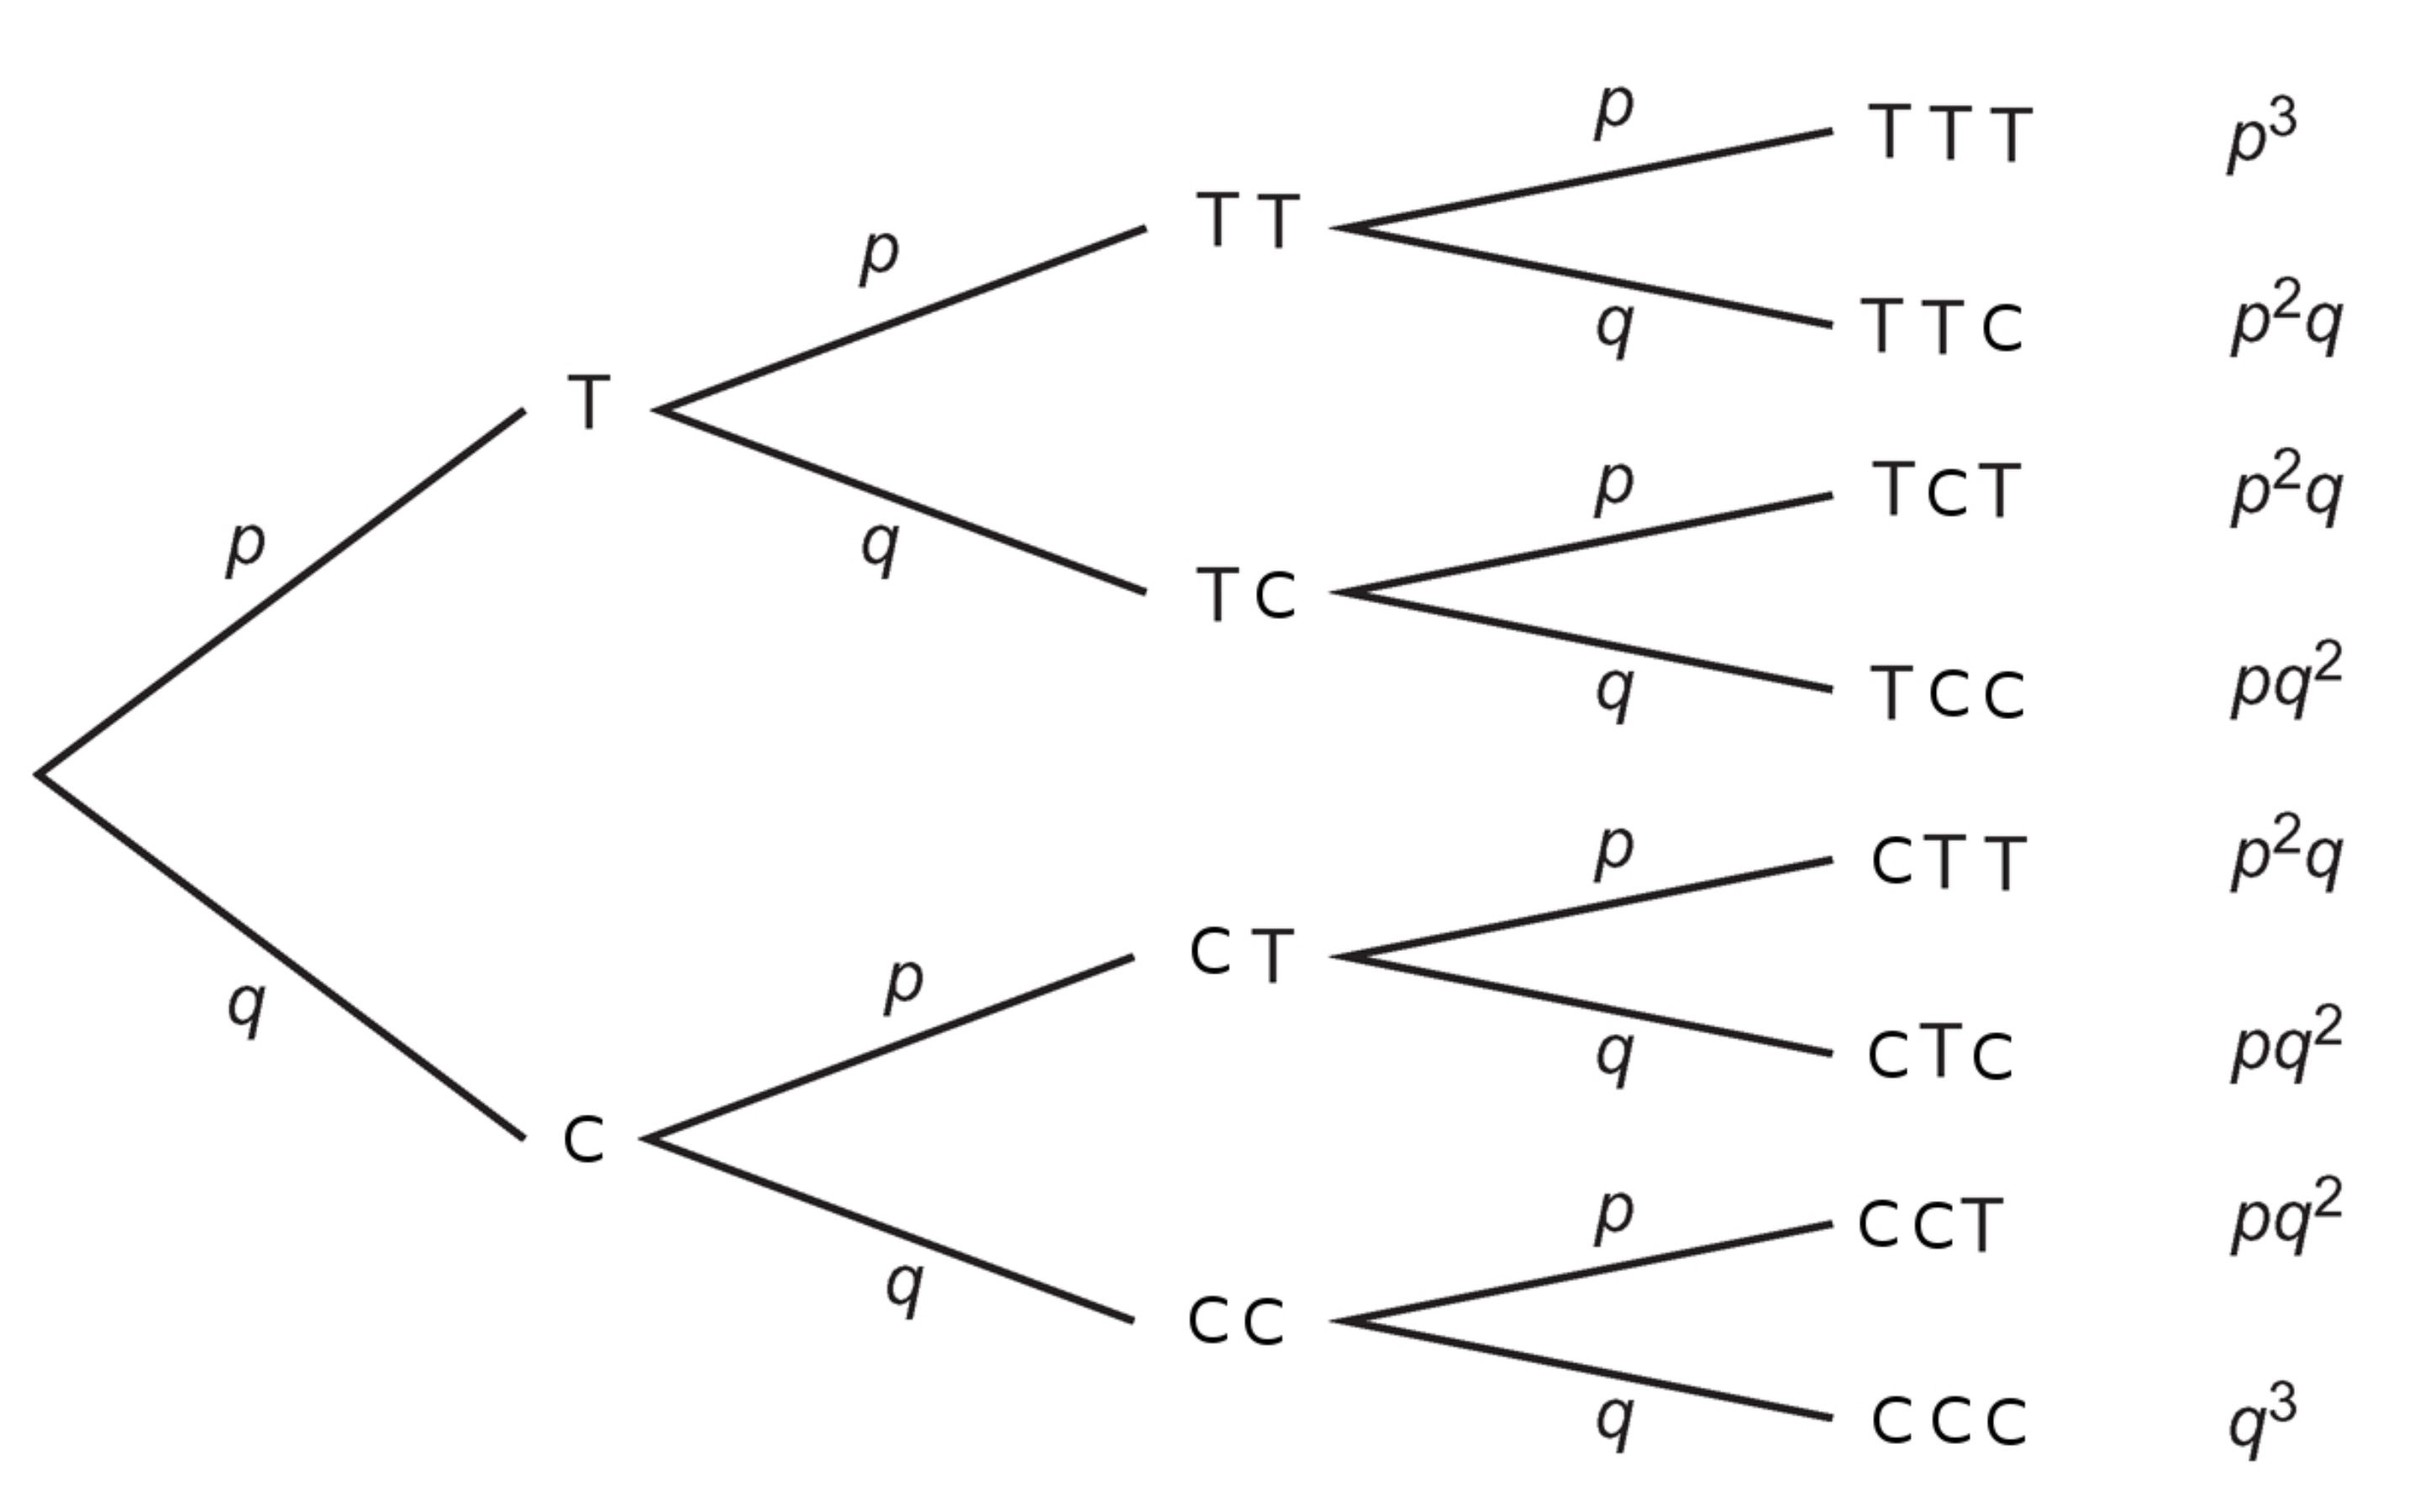
\includegraphics[width = 6.7cm]{img1.png}
  \caption{\textit{Diagramma ad albero per N=3}}
  \label{Fig1}
\end{figure}
\\
Quando, però, il numero di eventi cresce, costruire diagrammi di questo tipo risulta sconveniente. Passiamo quindi ad utilizzare il formalismo matematico per rissumere quello che accade.
\\Per definzione sappiamo che $p + q = 1$, ma allora:
$$(p+q)^N = 1$$
$$(p+q)^N = p^N + \frac{1}{2}N(N-1)p^{N-1}q + \dots + q^N$$
Utilizzando il binomio di Newton:
$$(p+q)^N = \sum_{M=0}^N \binom{N}{M} p^{N-M}q^M = \sum_{M=0}^N P(N;N-M)$$
Dove il coefficente binomiale è definito come:
$$\binom{N}{M} = \frac{N!}{M!(N-M)!}$$
e $P(N;N-M)$ è la probabilità di ottenere $N-M$ teste ed $M$ croci. Se ridefinissimo quindi $N_C$ come il numero di croci ($N_C = M$) e $N_T$ come il numero di teste ($N_T = N-M$), allora $P(N;N-M)$ diventa:
$$P(N;N-M) = P(N; N_T) = \binom{N}{M} p^{N-M}q^M = \frac{N!}{N_C!N_T!}p^{N_T}q^{N_C}$$
Nel caso della moneta è interessante osservare la devianza relativa tra $N_C$ ed $N_T$:
$$\frac{\Delta N}{N} = \frac{N_C-N_T}{N}$$
notando che tale grandezza tenderà a zero all'aumentare del numero dei lanci.
\\Una funzione $P(X)$ come quella appena definita viene detta distribuzione di probabilità, questa potra assumere valori discreti o continui a seconda del fenomeno osservato. In entrambi i casi è possibile definire dei valori che caratterizzano le proprietà della distribuzione in oggetto, quello che cambia è come questi valori verranno definiti. Nel caso di una distribuzione discreta si avranno:
\begin{enumerate}
  \item Valor Medio: $\langle x \rangle = \frac{1}{N}\sum_{i=0}^Nx_i$
\end{enumerate}
